\documentclass[10pt,reqno]{beamer}
\usepackage[utf8]{inputenc}
\usetheme{Dresden}
\usecolortheme{beaver}
\usepackage{amsmath}
\usepackage{amsfonts}
\usepackage{graphicx}
\usepackage{stmaryrd}
\usepackage{siunitx}
\usepackage{subcaption}
\usepackage[backend=biber, style=chem-acs]{biblatex}
\setbeamertemplate{navigation symbols}{} 
\title{Bond Graph Clinic: Part 3}
\subtitle{Biomolecular Systems}
\author{Peter Cudmore}

\institute{Systems Biology Lab, The University of Melbourne}

\newcommand{\D}[2]{\frac{\mathrm{d} #1}{\mathrm{d} #2}}
\newcommand{\e}{\mathrm{e}}
\newcommand{\I}{\mathrm{i}}
\renewcommand{\mod}[1]{\left|#1\right|}
\newcommand{\DD}[2]{\frac{\mathrm{d}^2 #1}{\mathrm{d} #2^2}}
\newcommand{\bigO}[1]{\text{O}\left(#1\right)}
\renewcommand{\P}[2]{\frac{\partial #1}{\partial #2}}
\renewcommand{\Re}{\operatorname{Re}}
\renewcommand{\Im}{\operatorname{Im}}
\newcommand{\EX}{\mathbb{E}}
\newcommand{\df}[1]{\mspace{2mu}  \mathrm{d}#1}
\newcommand{\reals}{\mathbb{R}}
\newcommand{\complex}{\mathbb{C}}
\newcommand{\conj}[1]{\overline{#1}}
\bibliography{references}

\begin{document}
	\begin{frame}
	\titlepage
	\addtocounter{framenumber}{-1} 
\end{frame}
\begin{frame}
\tableofcontents[hideallsubsections]
\end{frame}
\section{Introduction}
\subsection{Previously...}
\begin{frame}
\frametitle{Network models of energetic systems}
\begin{figure}
	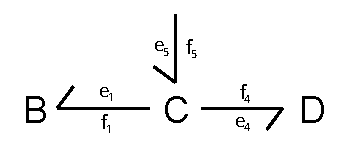
\includegraphics{images/bondgraph.pdf}
\end{figure}
Bond Graphs capture:
\begin{itemize}
	\item Energy transferred between $B,C,D$ without loss via bonds.
	\item Power transfer represented by conjugate variables $P_i=e_if_i$.
	\item Subsystem dynamics via constitutive relations $\Phi_B(e,f) = 0$
\end{itemize}
We've also looked at some examples.
\end{frame}
\begin{frame}
\frametitle{A Mathematicians Model of a Chemical System}
A naive description of molecular systems is as follows:
\begin{enumerate}
	\item A set of distinct quanta (molecules, complexes, atoms and free electrons) $A, B, \ldots$ move stochastically through a volume.
	\item When $A, B$ are sufficiently close they may bind to form complex $C$.
	\item After some time $\tau$, $C$ may disassociate into a number of quanta $E, \ldots$.
\end{enumerate}
All basic reaction types (synthesis, decomposition and replacement) can be represented in this way.\\
\vspace*{10pt}
Clearly this is an example of a \emph{reaction-diffusion} process.
\end{frame}
\subsection{Today}
\begin{frame}
\frametitle{This Clinic}
Today we shall consider \emph{reactions}.
\vfill

Next clinic will consider \emph{diffusion}.

\vfill

%For more details to Oster, Perelson and Auslander \cite{Oster:1971aa, Oster:1971ab, Oster:1973aa, Oster:1974aa, Perelson:1974, Auslander:1972aa}
\end{frame}
\begin{frame}
\frametitle{Spatial Assumptions}
Consider chemical reactions inside some vessel of fixed volume.\\
We assume that the chemical solution is well mixed, ie:
\begin{itemize}
	\item The solution is actively stirred or,
	\item the diffusion rate across the volume is orders of magnitude faster than the fastest reaction rate.
\end{itemize}
\vfill
This basically means we can work with average concentration, and ignore spatial effects inside the vessel.
\vfill
Later, we will couple many vessels together to represent diffusion.
\end{frame}
\section{Chemical Reactions}
\subsection{Chemical Reaction Networks}
\begin{frame}
\frametitle{Chemical Reaction Network: Petri Net}
\begin{figure}
	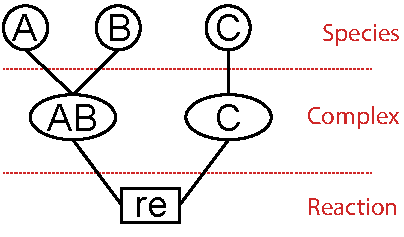
\includegraphics{images/petrinet_abc}
	\caption{Petri net of $A+B \rightleftharpoons C$}
\end{figure}
\end{frame}
\begin{frame}
\frametitle{Chemical Reaction Network: Bond Graph}
\begin{figure}
	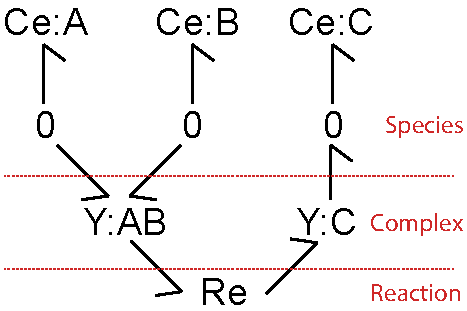
\includegraphics{images/bondgraph_abc}
	\caption{Bond Graph of $A+B \rightleftharpoons C$}
\end{figure}
\end{frame}


\begin{frame}
\frametitle{Thermodynamic Assumptions}
Consider chemical reactions inside some vessel of fixed volume.\\
We assume that the solution is \emph{isobaric} and \emph{isothermic}.
These assumptions allow us to define the chemical potential
\[
\mu_A = \mu_A^\varoslash + RT\ln \frac{x_A}{V_m}
\]
\only<1>{
\begin{itemize}
	\item $R=N_Ak_b\approx 8.314$ is the gas constant in \si{\joule\per\kelvin\per\mole}
	\item $T\approx 300$ is temperature (in \si{\kelvin})
	\item $\mu_A^\varoslash$ is the chemical potential of a pure solution of $A$ in \si{\joule}
	\item $x_A$ the amount of species $A$ in \si{\mole}.
	\item $V_m$ is volume of the solution in \si{\mole}
\end{itemize}
This follows from the \emph{Ideal Gas Law} and the \emph{Fundamental Equation of Thermodynamics}.
}
\only<2>{
\begin{align*}
\text{Energy}&=x_A \cdot \mu_A \si{\joule} \\
\text{Power}&=\dot{x}_A\cdot \mu_A\ \si{\joule\per\second}
\end{align*}
\begin{center}
$\mu_A$ is \emph{effort} or force-like \\
\vspace{10pt}
$\dot{x}_A$ is the \emph{flow} or flux-like.
\end{center}
\vfill
}

\only<3>{
Recall $x_A$ is the molar amount of species $A$.\\
\vfill 
Question:\\
What happens to $\mu_A$ when $x_A \rightarrow 0$ but $V_m$ is constant?\\
When might this occur and is this physical?
}
\end{frame}
\subsection{Components}
\begin{frame}
\frametitle{Ce Constitutive Relation}
\begin{figure}
	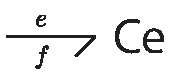
\includegraphics{images/oneport-Ce.pdf}
\end{figure}
Constitutive Relation for a Chemical Species:
\[
\Phi_{Ce}(e,f) = e - \beta \ln kq = 0 
\]
\vfill
\only<2>{
This follow from substituting the parameters 
\[
k = \exp(\mu_A^\varoslash/RT)/V_m,\qquad \beta = RT
\]
and the state variables $\mu_A = e$, $\dot{x}_A = f$ and $x_A = q  = q_0 + \int_0^t f\df{t} $ into 
\[
\mu_A = \mu_A^\varoslash + RT\ln \frac{x_A}{V_m}.
\]}
\only<3>{
\[
\beta = RT, \qquad k = \exp(\mu_A^\varoslash/\beta)/V_m
\]
\vfill
\begin{center}
\emph{It will often be convenient for us to take $\beta =1$}
\end{center}
}
\end{frame}
\begin{frame}
\frametitle{Chemical Kinetics}
Reactions proceed according to the \emph{Marcelin-de Donder} formula
\[
v = \kappa\left(\e^{A^f/RT} - \e^{A^r/RT}\right)
\]
\only<1>{Here:
\begin{itemize}
	\item $v$ is the reaction velocity or molar flow
	\item $A^f, A^r$ are the forward and reverse chemical affinities
	\item $\kappa$ is the reaction rate constant.
	\item $R,T$ is the gas constant and temperature respectively.
\end{itemize}}
\only<2>{

The mass flow in is $v$, hence the mass flow out is $-v$.\\
\vspace{10pt}
So
\[
f_1 = v,\qquad f_2 = -v
\]
are natural \emph{flow} variables.

}
\only<3>{

For a chemical reaction $\nu^f_AA + \nu^f_BB +\ldots \rightleftharpoons \nu^f_AA + \nu^f_BB +\ldots$ with forward and reverse stoichiometric coefficients $\nu^f$ and $\nu^r$.\\
\vfill
The forward (and similarly reverse) affinity is defined as
\[
A^f = \nu^f_A\mu_A + \nu^f_B\mu_B +\ldots
\]
So the natural effort variables are
\[
e_1 =  A^f, \qquad e_2 = A^r.
\]
}
\end{frame}
\begin{frame}
\frametitle{Re Constitutive Relation}
\begin{figure}
	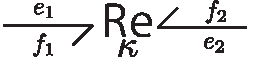
\includegraphics{images/twoport-Re.pdf}
\end{figure}
Constitutive Relation for a reaction component:
\[
\Phi_{Re}(\mathbf{e},\mathbf{f}) = \left(
\begin{matrix}
\kappa[\exp(\e_1/\beta) - \exp(\e_2/\beta)] - f_1\\
f_1 + f_2
\end{matrix}
\right) = 0
\]
\vfill
\only<1>{
Where again $\beta =RT$ is often taken as $\beta =1$.
}
\only<2>{
This follows directly from the Marcelin-de Donder formula.
}
\end{frame}
\begin{frame}
\frametitle{Putting it together}
\begin{figure}
	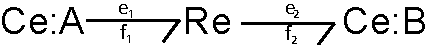
\includegraphics{images/bondgraph_ab}
\end{figure}
{\scriptsize
The above bond graph describes the reaction $A\rightleftharpoons B$.

\begin{minipage}{0.475\linewidth}
\begin{align}
\Phi_{Ce:A} &= e_1 - \ln k_A\left[q_A(0)  + \int(- f_1)\df{t}\right]\\
\Phi_{Ce:B} &= e_2 - \ln k_B\left[q_B(0)  + \int f_2\df{t}\right]
\end{align}
\end{minipage}\hfill
\begin{minipage}{0.475\linewidth}
\begin{align}
\Phi_{Re}(\mathbf{e},\mathbf{f}) &= \left(
\begin{matrix}
\kappa\left[\e^{e_1} - \e^{e_2}\right] - f_1\\
f_1 +(- f_2)
\end{matrix}
\right)
\end{align}	
\end{minipage}
\vspace{11pt}

Recall that $q(t) = q_0 + \int_0^t f(t)\df{t}$. So define 
\begin{align*}
\dot{x}_A  = \dot{q_1} &= -f_1 &\implies&& q_1 &= q_A(0) -\int_0^t f_1 \df{t} &\implies &&\e^{e_1} &= k_Aq_1, \\
\dot{x}_B = \dot{q_2} &= f_2 &\implies&& q_2 &= q_B(0) +\int_0^t f_2 \df{t} &\implies &&\e^{e_2} &= k_Bq_2.
\end{align*}

The second line of (3) gives $f_1 = f_2$ which implies $-\dot{q_1} = \dot{q_2}$, and the first gives the result
\[
\dot{q_1} = - \kappa\left(k_Aq_1 - k_Bq_2\right) = k_-q_2 - k_+q_1 \quad \text{where}\quad k_+ = \kappa k_A,\ k_- =\kappa k_B.
\]

}
\end{frame}

\section{Stoichiometry}
\begin{frame}
\frametitle{Complexes}
The reaction $A + B \rightleftharpoons C$ can be though of
\begin{enumerate}
	\item $A$ and $B$ collide forming a complex $AB$.
	\item $AB$ reacts to form $C$. 
\end{enumerate}
\vfill

Clearly, the flow of $A$ and the flow of $B$ into this reaction are equal.
\vfill

Hence, we \emph{should} be able to represent the $AB$ complex as a equal flow junction, and allow the reaction to drive what that flow is.

\begin{center}
\textbf{Just using the usual common flow 1 junction wont work!}\\
\vspace{10pt}
\emph{Question: Why?}
\end{center}
\end{frame}

\begin{frame}
\frametitle{Naive example: $A+B\rightleftharpoons B$}
\begin{figure}
	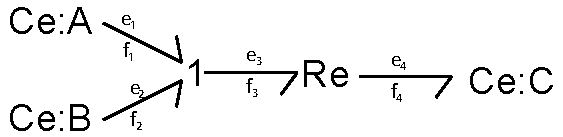
\includegraphics[scale=0.8]{images/bondgraph_abc_naive}
\end{figure}
{\scriptsize
\begin{minipage}{0.475\linewidth}
\begin{align}
\Phi_{Ce:A} &= e_1 - \ln k_A(q_1),\\
\Phi_{Ce:B} &= e_2 - \ln k_B(q_2),\\
\Phi_{Ce:B} &= e_2 - \ln k_C(q_3)
\end{align}
\end{minipage}
\begin{minipage}{0.475\linewidth}
	\begin{align}
\Phi_{Re} &= \left(
\begin{matrix}
	\kappa\left[\e^{e_3} - \e^{e_4}\right] - f_3\\
	f_3 + (- f_4)
\end{matrix}
\right),\\
\Phi_1(\mathbf{e},\mathbf{f})&=\left(
\begin{matrix}
	e_1 + e_2 + e_3\\
	f_1 - (-f_3)\\
	f_2- (-f_3)\end{matrix}\right),
\end{align}
\end{minipage}	

From the first equation of (8) we have
\[
e_3 = -(e_1 + e_2) \implies f_3 = \kappa \left(\e^{ - e_1 - e_2} - \e^{e_4}\right) = \kappa\left(\frac{1}{k_A k_Bq_1 q_2} + k_Cq_3\right)
\]
Which is clearly wrong as we should not be able to get inverse powers!}
\end{frame}
\begin{frame}
\frametitle{What when wrong}
We're actually coupling two slightly different thermodynamic domains;
\begin{itemize}
	\item \emph{chemical potential energy} (that is, the stored in a heterogeneous solution)
	\item \emph{chemical reaction affinity} (the energy stored in a complex).
\end{itemize}

These overlap only when the species IS the complex; hence why it works for the reaction $A\rightleftharpoons B$.
\vspace{10pt}

What we need is a mapping between species space and complex space.

\end{frame}

\begin{frame}
\frametitle{Stoichiometry}
\begin{figure}
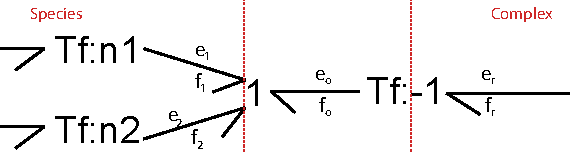
\includegraphics{images/stoic_oster}
\end{figure}

Oster \emph{et. al.}~\cite{Oster:1973aa} represented reaction stoichiometry using the above bond graph.
\\
Here $n1$ and $n2$ are the number of molecules of species $1$ and $2$ consumed by the reaction. 
\vspace{10pt}

Recall that 
$\Phi_{TF:\rho}(e_j, f_j, e_k,f_k) = 0 \implies e_k =  \rho e_j,\qquad f_k = \rho^{-1}f_j$ and 
hence
\[
e_r = -e_o, \qquad e_1 = n_1\mu_1,\qquad e_2 = n_2\mu_2.
\]

Since $e_1 +e_2 +e_o  =0$ it follows that the reaction affinity is
\[
A^f =e_r = -e_o = e_1 + e_2 = n_1\mu_1 + n_2 \mu_2
\]
\end{frame}
\begin{frame}
\frametitle{Gawthrop's Reduction}
\begin{figure}
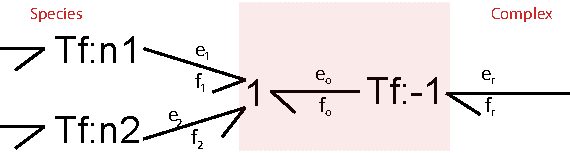
\includegraphics[scale=0.5]{images/stoic_oster_A}
\end{figure}
\begin{center}
Gawthrop~\cite{Gawthrop:2014aa} replace the shaded box with the\\ \emph{biochemical 1 junction} defined by 
\end{center}

\begin{figure}
	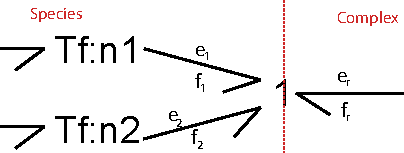
\includegraphics[scale=0.5]{images/stoic_gaw}
\end{figure}
\[
\Phi_{1} = \left(\begin{matrix}
e_o - (e_1 +e_2)\\
f_o -f_1\\
f_o -f_2  
\end{matrix}\right) = 0\implies f_r = -f_1 = -f_2, \quad e_r= e_1 + e_2
\]
\end{frame}
\begin{frame}
\frametitle{An alternative}
An alternative would be to replace
\begin{figure}
	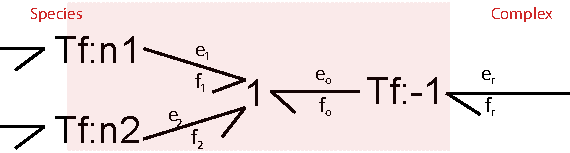
\includegraphics[scale=0.5]{images/stoic_oster_Y}
\end{figure}
\begin{center}
with
\end{center}
\begin{figure}
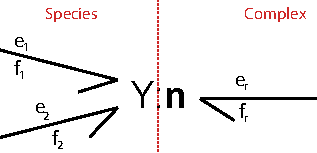
\includegraphics[scale=0.5]{images/stoic_Y}
\end{figure}
Where $\mathbf{n}$ is the forward or reverse (truncated) stoichiometric vector which in this case $\mathbf{n} = (n_1,n_2)$.
\end{frame}
\subsection{Through Junction}
\begin{frame}
\frametitle{Through Junction}
\begin{minipage}{0.58\textwidth}
\begin{figure}
	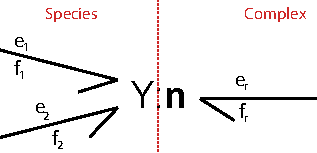
\includegraphics{images/stoic_Y}
\end{figure}
\end{minipage}
\begin{minipage}{0.38\textwidth}
Constitutive Relation:
\[
\Phi_{Y} = \left(\begin{matrix}
e_r - \sum n_ie_i \\
f_r + \frac{f_1}{n_1}\\
\vdots
\end{matrix}\right)
\]
\end{minipage}

\vspace{20pt}
\only<1>{

$\text{Y}$ is power conserving. Multiplying the top line by $f_r$ gives 
\[
0 = e_r f_r - f_r\sum e_i n_i  =e_r f_r - \sum e_i (n_if_r)
\]
Since $n_if_r = -f_i$, the result follows from
\[
0 = e_r f_r - \sum e_i (n_if_r) = e_rf_r + \sum e_if_i.
\]
This is no surprise as $\text{Y}$ is built from conserving components.
}
\only<2>{\begin{center}
The through junction	$\text{Y}$ 
	\begin{itemize}
		\item is power conserving,
		\item is unambiguous,
		\item is symbolically consistent,
		\item maps cleanly on existing C.R.N. theory.
	\end{itemize}
\end{center}
}
\end{frame}
\begin{frame}
\frametitle{$A+B\rightleftharpoons C$: redux.}
{\scriptsize
\begin{figure}
	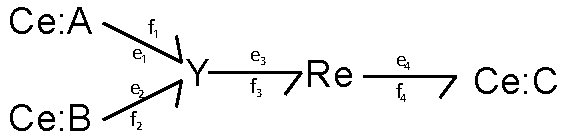
\includegraphics[scale=0.5]{images/bondgraph_abc_final}
	\caption{Bond Graph of $A+B \rightleftharpoons C$}
\end{figure}
\begin{minipage}{0.475\textwidth}
\begin{align}
\Phi_{Ce:A} &= e_1 - \ln k_A(q_1),\\
\Phi_{Ce:B} &= e_2 - \ln k_B(q_2),\\
\Phi_{Ce:B} &= e_2 - \ln k_C(q_3)
\end{align}
\end{minipage}
\begin{minipage}{0.475\textwidth}
\begin{align}\Phi_{Re} &= \left(
\begin{matrix}
\kappa\left[\e^{e_3} - \e^{e_4}\right] - f_3\\
f_3 + (- f_4)
\end{matrix}
\right),\\
\Phi_{Y} &= \left(\begin{matrix}
e_3 - e_1 - e_2 \\
(-f_3) + f_1\\
(-f_3) + f_2\\
\end{matrix}\right)
\end{align}
\end{minipage}

\vfill
Clearly
\[
e_3 = e_1 + e_2 \implies \exp(e_3) = \exp(\ln k_A q_1 + \ln k_Bq_2) = k_Ak_B q_1q_2.
\]
Since $f_4 = \dot{q_4}$,  it follows from (12) that
\[
\dot{q_4} =  \kappa k_Ak_B q_1q_2 - \kappa k_C q_4 = k_+q_1q_2 - k_-q_4.
\]
From (12) and (13) we have $\dot{q_4} = f_4 =f_3= f_2 = f_1$.\\
Combining this with $f_1 = -\dot{q_1} $ and $f_2 = -\dot{q_2}$ completes the picture.
}
\end{frame}
\begin{frame}
\frametitle{$A+B\rightleftharpoons C$: final form!}
\begin{figure}
	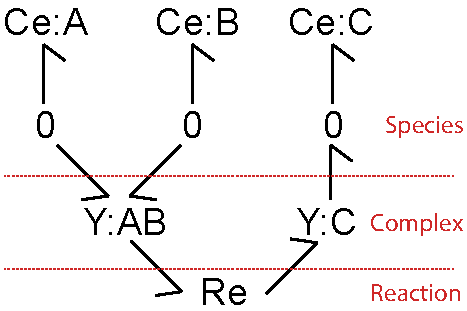
\includegraphics[scale=0.75]{images/bondgraph_abc}
	\caption{Bond Graph of $A+B \rightleftharpoons C$}
\end{figure}
In the above figure we have added standard 0 junctions. While this is redundant in this above reaction, it allows us to use the same species for many reactions.
Also, note that $\text{Y:C}$ is the identity (\emph{prove it!}) and may be omitted.
\end{frame}
\section{Conclusion}
\begin{frame}
\frametitle{In Review}
\begin{figure}
	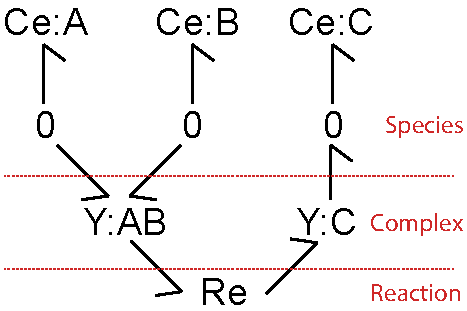
\includegraphics[scale=0.75]{images/bondgraph_abc}
	\caption{Bond Graph of $A+B \rightleftharpoons C$}
\end{figure}
\only<1>{
The $\text{Ce}$ is a one port component representing a store of a particular chemical species and has a constitutive relation that captures the usual definition of \emph{chemical potential energy}.
}
\only<2>{
The zero junctions allow species A B and C to be share across reactions other than the one modelled in this graph.
}
\only<3>{
The $\text{Y}$ component is a power conserving through junction, which captures the forward (in the case of $\text{Y:AB}$) and reverse stoichiometry of this reaction.
}
\only<4>{
The $\text{Re}$ component models how the complex $A+B$ transmutes into $C$. The reaction proceeds according to the \emph{Marcelin-de Donder} formula.
}
\end{frame}

\begin{frame}
\frametitle{Try for yourself}
Try drawing bond graphs of these common reactions:
\begin{itemize}
	\item $A+B \rightleftharpoons D+C$
	\item $A+B \rightleftharpoons B+C$
	\item $E + S \rightleftharpoons ES \rightleftharpoons E+P$
\end{itemize}
\vfill
{\scriptsize
	\begin{minipage}{0.475\textwidth}
		\begin{align*}
		\Phi_{Ce}(e,f) &= e - \ln k(q),\\
		\Phi_{Re}(e_f,f_f,e_r,f_r) &= \left(
		\begin{matrix}
		\kappa\left[\e^{e_f} - \e^{e_r}\right] - f_f\\
		f_f +  f_r
		\end{matrix}
		\right)\\
		\Phi_{Y}(e_0,f_0, e_1,f_1,\ldots) &= \left(\begin{matrix}
		e_0 - \sum n_ie_i \\
		f_0 + f_i/n_i\\
		\vdots
		\end{matrix}\right)
		\end{align*}
	\end{minipage}
\begin{minipage}{0.475\textwidth}
	\raggedright
	\begin{figure}
	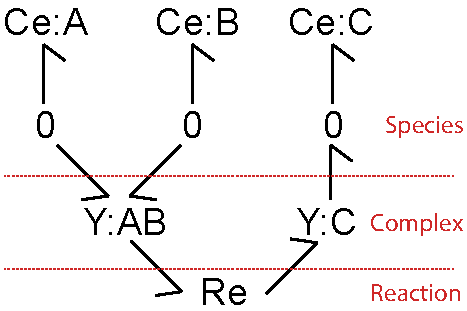
\includegraphics[width=0.75\linewidth]{images/bondgraph_abc}
	\end{figure}
\end{minipage}
	

}
\end{frame}
\begin{frame}
\frametitle{References}
\printbibliography
\end{frame}

\end{document}